% LUCA — LLM-based Unified Corporate Analyst
% Paper (AI Lab). IEEEtran, doble columna, en español.
% Figuras y tabla de resultados regeneradas por experiments/make_figures.py.
\documentclass[conference]{IEEEtran}

\usepackage[utf8]{inputenc}
\usepackage[T1]{fontenc}
\usepackage{graphicx}
\usepackage{booktabs}
\usepackage{amsmath}
\usepackage{amssymb}
\usepackage{url}
\usepackage{hyperref}

\graphicspath{{figures/}}

% El paquete babel-spanish no está disponible en esta distribución TeX. El
% cuerpo se compone correctamente en español vía inputenc UTF-8; aquí solo
% traducimos las etiquetas estructurales de IEEEtran al español.
\renewcommand{\abstractname}{Resumen}
\renewcommand{\refname}{Referencias}
\providecommand{\IEEEkeywordsname}{Términos índice}
\renewcommand{\IEEEkeywordsname}{Términos índice}

% Macros del corpus (auto-generadas desde experiments/corpus_manifest.csv
% por experiments/make_corpus_tables.py; no editar a mano).
% AUTO-GENERATED by experiments/make_corpus_tables.py — do not edit by hand.
% Source: corpus_manifest.csv (288 rows, 96 companies).
% Input this file in the preamble; corpus_tables.tex goes in the appendix.
\newcommand{\corpusFilings}{288}
\newcommand{\corpusCompanies}{96}
\newcommand{\corpusCoverage}{95.7}


\begin{document}

\title{LUCA: un pipeline multiagente híbrido XBRL--LLM para la\\
generación automática de \textit{investment memos} de informes 10-K\\
en hardware de consumo}

\author{\IEEEauthorblockN{Ignacio Queipo de Llano Pérez-Gascón}
\IEEEauthorblockA{ICAI, Universidad Pontificia Comillas\\
Madrid, España\\
\texttt{iqueipo.pg24@gmail.com}}
% Para añadir tutor,
% descomenta y rellena el bloque siguiente:
% \and
% \IEEEauthorblockN{<Nombre del tutor>}
% \IEEEauthorblockA{ICAI, Universidad Pontificia Comillas\\Madrid, España}
}

\maketitle

\begin{abstract}
LUCA (\textit{LLM-based Unified Corporate Analyst}) es un pipeline multiagente que ingiere un documento financiero regulatorio
(un informe 10-K de SEC EDGAR) y produce un \textit{investment memo}
estructurado. Su decisión de diseño central es la extracción \emph{híbrida}: las
cifras numéricas se obtienen de los datos XBRL del propio documento (sin LLM,
exactas y deterministas), mientras que el modelo de lenguaje, un Qwen~2.5 7B
cuantizado a Q4\_K\_M servido localmente con Ollama, se reserva únicamente para
el contenido cualitativo (riesgos, discusión y \textit{outlook}). Todo el
sistema se ejecuta en una única GPU de consumo (RTX~4060, 8\,GB) y no emplea
modelos externos ni APIs de pago en ninguna etapa. Sobre un \textit{gold
standard} anotado manualmente de 60 puntos de dato (6 métricas $\times$ 10
empresas), el extractor estructurado alcanza un 100\% de precisión
(determinista), frente al 50.0--51.7\% del mejor baseline LLM (no determinista
entre ejecuciones) y un 3.3\% de un baseline LLM ingenuo; una brecha de
$\approx$48--50~puntos porcentuales (pp) que motiva la arquitectura híbrida. En
la capa cualitativa, validamos manualmente la extracción de riesgos contra los
informes originales y documentamos un patrón de sobre-extracción no uniforme,
que constituye un resultado honesto sobre los límites de un modelo de 7B en
hardware de consumo.
\end{abstract}

\begin{IEEEkeywords}
extracción financiera, XBRL, modelos de lenguaje, sistemas multiagente,
hardware de consumo, 10-K, alucinación numérica.
\end{IEEEkeywords}

\section{Introducción}
El análisis de informes financieros regulatorios es una tarea intensiva en
conocimiento experto. Un informe anual 10-K de la \textit{Securities and
Exchange Commission} (SEC) estadounidense supera con frecuencia los dos millones
de caracteres de HTML y combina estados financieros consolidados, una sección de
factores de riesgo (Item~1A) y una discusión de la dirección (Item~7). Extraer
de forma fiable las magnitudes numéricas y sintetizar el contenido cualitativo
es el trabajo que realiza un analista junior, y un candidato natural a la
automatización.

Un \textit{investment memo} sintetiza ese trabajo en un documento estructurado:
un resumen ejecutivo, una visión del negocio, los aspectos financieros con sus
cifras clave, un análisis de riesgos y unas perspectivas. Producirlo a mano para
una sola empresa lleva horas de lectura y tabulación, y el cuello de botella no es
el juicio analítico sino la extracción fiable de magnitudes y la lectura de
secciones extensas como los factores de riesgo. Automatizar esa capa de extracción
y síntesis, conservando la trazabilidad hasta el documento fuente, es el objetivo
de LUCA.

Las aproximaciones recientes basadas en grandes modelos de lenguaje (LLM)
presentan dos modos de fallo en este dominio. Por un lado, los enfoques
\emph{LLM-only}, que entregan el documento al modelo y le piden que extraiga las
cifras, son frágiles: el modelo alucina valores numéricos, confunde columnas de
ejercicios adyacentes y mezcla magnitudes consolidadas con atribuibles. La
literatura de evaluación de alucinación~\cite{ji2023hallucination} y los
benchmarks de razonamiento numérico financiero~\cite{chen2021finqa,zhu2021tatqa}
documentan ampliamente esta limitación. Por otro lado, los sistemas que sí
alcanzan precisión de grado experto suelen depender de modelos propietarios de
gran tamaño servidos tras APIs comerciales cerradas~\cite{wu2023bloomberggpt},
lo que introduce coste por consulta, dependencia de un proveedor y envío de
datos a terceros.

Este trabajo parte de una restricción deliberada y verificable: \emph{todo el
sistema debe ejecutarse en hardware de consumo} (una GPU RTX~4060 de 8\,GB) con
un modelo abierto y cuantizado servido localmente, sin ninguna llamada a
servicios de pago. La pregunta de investigación que abordamos es: \textit{¿puede
un pipeline multiagente sobre hardware de consumo, usando un modelo de 7B local
solo allí donde aporta valor, igualar la precisión numérica de un experto al
mismo tiempo que produce un memo cualitativo utilizable?}

Nuestra respuesta es una arquitectura híbrida en la que la división del trabajo
entre componentes deterministas y el LLM es explícita. Las contribuciones del
trabajo son tres:

\begin{enumerate}
  \item \textbf{Una arquitectura híbrida XBRL+LLM} en la que las cifras provienen
  de los \textit{facts} XBRL del documento (sin LLM, exactas) y el modelo de 7B
  local se limita al texto cualitativo. Esto es lo que hace viable ejecutar el
  pipeline completo en 8\,GB de VRAM.
  \item \textbf{Una comparación empírica de precisión} frente a dos baselines
  LLM-only (ingenuo y estructurado), sobre un \textit{gold standard} anotado a
  mano, que cuantifica la ventaja de la extracción estructurada
  (Tabla~\ref{tab:accuracy}).
  \item \textbf{Un análisis honesto del techo de calidad} del modelo de 7B en la
  parte cualitativa, incluyendo un patrón de sobre-extracción de riesgos validado
  manualmente contra los informes originales y reportado como limitación.
\end{enumerate}

LUCA es un proyecto de \textit{AI Lab} que reutiliza, en el dominio financiero,
la arquitectura multiagente de un sistema previo orientado a revisiones
sistemáticas. El interés metodológico de este traslado es comprobar que la misma
descomposición en agentes especializados, con una frontera explícita entre
componentes deterministas y generativos, generaliza a otro dominio intensivo en
documentos. El resto del artículo se organiza así: la
\S\ref{sec:architecture} describe la arquitectura; la \S\ref{sec:impl}, la
implementación y las pruebas; la \S\ref{sec:experiments}, la metodología de
evaluación; la \S\ref{sec:results}, los resultados; la \S\ref{sec:discussion}, la
discusión; y la \S\ref{sec:future}, el trabajo futuro.

\section{Trabajo relacionado}
\textbf{LLMs en el dominio financiero.} BloombergGPT~\cite{wu2023bloomberggpt}
demostró las ventajas de un modelo de 50B entrenado sobre un corpus financiero
masivo, pero su escala y su carácter propietario lo sitúan fuera del alcance del
hardware de consumo. En el extremo de los modelos especializados ligeros,
FinBERT~\cite{araci2019finbert} adaptó BERT al análisis de sentimiento
financiero. Los benchmarks FinQA~\cite{chen2021finqa} y TAT-QA~\cite{zhu2021tatqa}
formalizaron el razonamiento numérico sobre datos financieros tabulares y
textuales, y evidenciaron que la extracción de cifras exactas es un punto débil
persistente de los modelos generativos. Estos benchmarks, sin embargo, plantean
preguntas sobre tablas o fragmentos ya seleccionados, mientras que LUCA opera
sobre el documento 10-K completo, donde el reto incluye \emph{localizar} la cifra
correcta en cientos de miles de caracteres antes de leerla. Nuestro resultado del
baseline ingenuo muestra que ese problema de localización, y no solo el de
lectura, es crítico cuando no se dispone de un acceso estructurado a los datos.

\textbf{Alucinación y fiabilidad numérica.} El estudio de Ji
\textit{et~al.}~\cite{ji2023hallucination} ofrece una taxonomía de la alucinación
en generación de lenguaje natural. En extracción financiera, la alucinación de
una sola cifra invalida un memo completo, lo que motiva nuestra decisión de no
delegar números al LLM. Técnicas de \textit{prompting} como
\textit{chain-of-thought}~\cite{wei2022cot} mejoran el razonamiento, pero no
garantizan la exactitud de una magnitud copiada de un estado financiero.

\textbf{Sistemas multiagente con LLMs.} Marcos como
ReAct~\cite{yao2023react}, que entrelaza razonamiento y acción, y
AutoGen~\cite{wu2023autogen}, que orquesta múltiples agentes conversacionales,
han popularizado la descomposición de tareas complejas en agentes
especializados. LUCA adopta esta filosofía de descomposición, pero con una
diferencia metodológica clave: no todos los agentes usan el LLM; los agentes
numéricos son deterministas por diseño. Frente a los marcos en los que cada agente
es una instancia del LLM que conversa con las demás, LUCA traza una frontera
explícita entre lo que resuelve el dato estructurado y lo que resuelve el modelo,
y esa frontera es la que se evalúa en este trabajo.

\textbf{Modelos abiertos y locales.} La disponibilidad de modelos abiertos
competentes como la familia LLaMA~\cite{touvron2023llama} y
Qwen~2.5~\cite{qwen2025}, junto con la cuantización y los servidores locales de
inferencia, ha hecho viable ejecutar modelos de 7B en GPUs de consumo. LUCA se
apoya en esta línea: emplea Qwen~2.5 7B cuantizado a Q4\_K\_M sobre Ollama, y
trata su capacidad limitada como una restricción del problema, no como un
defecto a ocultar.

\section{Arquitectura del sistema}
\label{sec:architecture}
LUCA se organiza como un pipeline de ocho agentes. La
Tabla~\ref{tab:agents} resume el rol y el estado de implementación de cada uno,
y la Fig.~\ref{fig:arch} muestra el flujo de datos y, mediante color, qué
agentes son deterministas y cuáles invocan el modelo de 7B local.

\begin{figure}[t]
\centering
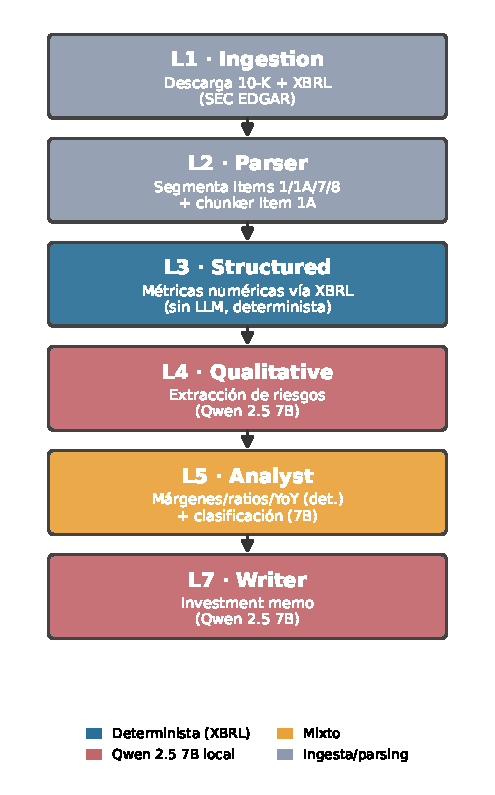
\includegraphics[width=0.93\linewidth]{fig_architecture.pdf}
\caption{Arquitectura del pipeline L1$\rightarrow$L7. El color distingue los
componentes deterministas (L3, vía XBRL) de los que invocan el Qwen~2.5 7B local
(L4, L7) y los mixtos (L5: aritmética determinista + clasificación con LLM).}
\label{fig:arch}
\end{figure}

\begin{table}[t]
\centering
\caption{Agentes de LUCA y su estado. ``Evaluado'' significa medido contra el
\textit{gold standard} (\S\ref{sec:experiments}).}
\label{tab:agents}
\small
\begin{tabular}{@{}lp{0.40\columnwidth}p{0.26\columnwidth}@{}}
\toprule
Agente & Rol & Estado \\
\midrule
L1 Ingestion & Descarga 10-K + XBRL (EDGAR) & Impl., evaluado \\
L2 Parser & Segmenta Items 1/1A/7/8 & Impl., evaluado \\
L2 \textit{chunker} & Troceado de Item 1A & Impl., evaluado \\
L3 Structured & Métricas numéricas (XBRL) & Impl., evaluado \\
L4 Qualitative & Extracción de riesgos & Impl. (parcial) \\
L5 Analyst & Métricas derivadas + clasif. & Impl. (parcial) \\
L7 Writer & \textit{Investment memo} (Qwen) & Impl. (demo AAPL) \\
L6 Comparables & Análisis comparado & Trabajo futuro \\
L8 Explainer & Excel + \textit{explainability} & Trabajo futuro \\
\bottomrule
\end{tabular}
\end{table}

\subsection{Principio híbrido}
La premisa que vertebra el diseño es que los datos numéricos deben provenir de
los \textit{facts} XBRL de \textit{companyfacts} (deterministas, gratuitos y
exactos), mientras que el LLM se restringe al texto cualitativo. Esta separación
no es solo una decisión de calidad: es lo que hace que el pipeline completo
quepa en 8\,GB de VRAM, porque el modelo de 7B nunca tiene que procesar los
megabytes de tablas financieras del documento.

\subsection{L1 -- Ingestion}
L1 resuelve el \textit{ticker} a su CIK mediante el mapa de la SEC, descarga el
\textit{submissions} JSON para localizar el 10-K más reciente, y obtiene tanto
el HTML del informe como el \textit{companyfacts} XBRL. Las descargas se cachean
en disco por \textit{(ticker, accession)} y se respeta el límite de tasa de
EDGAR. La salida es un diccionario con el HTML, los \textit{facts} XBRL, la fecha
de \textit{filing} y el número de \textit{accession} para trazabilidad.

\subsection{L2 -- Parser}
L2 convierte el HTML a texto plano y segmenta el documento en los Items 1, 1A, 7
y 8. La segmentación evita un error frecuente: anclar las secciones en el índice
(\textit{table of contents}) en lugar del cuerpo, lo que se resuelve detectando
el índice por su estructura DOM y exigiendo el título canónico de la SEC. Sobre
Item~1A actúa además un \textit{chunker} específico, descrito a continuación.

\subsection{L2b -- \textit{Chunker} de Item 1A}
La sección de factores de riesgo es demasiado larga para una sola ventana de
contexto, por lo que requiere un troceado que respete su estructura. Un hallazgo
de diseño relevante es que los 10-K en formato iXBRL no marcan los encabezados
con etiquetas semánticas (\texttt{<h1>}, \texttt{<b>}), sino con CSS en línea del
tipo \texttt{font-weight:700}. El \textit{chunker} detecta, por tanto, los
anclajes \textit{bold-leading}: el primer texto de un \texttt{<div>} cuyo ancestro
tiene \textit{font-weight} $\geq$600. Cada bloque del cuerpo queda delimitado por
anclajes consecutivos, de modo que se corresponde con un factor de riesgo del
documento.

Tres filtros anti-falsos-positivos descartan anclajes espurios: numéricos puros,
patrones de número de página, y encabezados repetidos tres o más veces en el
documento. Un heurístico adicional detecta el \textit{Risk Factor Summary} (un
encabezado corto seguido de al menos tres \textit{bullets} en los primeros 5\,000
caracteres) y lo marca con una bandera \texttt{in\_summary}, señal que la capa de
deduplicación de trabajo futuro podrá aprovechar. Por último, un bloque que excede
las 4\,000 \textit{tokens} ($\approx$16\,000 caracteres) se subdivide con un
solape de 500 caracteres, y un relleno de huecos garantiza la cobertura íntegra de
la sección.

\subsection{L3 -- Structured Extractor}
L3 es el corazón determinista del sistema y la fuente de todas las cifras del
memo. Para cada métrica canónica mantiene una cadena ordenada de etiquetas
US-GAAP candidatas (preferente primero, alternativas después) y selecciona el
\textit{fact} anual más reciente a lo largo de toda la cadena, con desempate por
prioridad de etiqueta. Filtra por formulario (\texttt{10-K}), periodo fiscal
(\texttt{FY}), unidad (USD o USD/acción) y duración ($\geq$320 días, para
rechazar trimestres etiquetados como anuales). Un \textit{guard} de recencia
(730 días respecto a la fecha de \textit{filing}) descarta etiquetas obsoletas
heredadas del histórico agregado de \textit{companyfacts}. L3 nunca usa el LLM y
nunca lanza excepción ante XBRL ausente: devuelve \texttt{None} y continúa.

Un ejemplo ilustra por qué la selección recorre toda la cadena en lugar de
detenerse en la primera etiqueta. Para los ingresos de Apple, la etiqueta
heredada \texttt{Revenues} conserva en \textit{companyfacts} un \textit{fact}
obsoleto de FY2017, mientras que la cifra vigente bajo ASC-606 vive en
\texttt{RevenueFromContract\-\allowbreak WithCustomer\-\allowbreak ExcludingAssessedTax}.
Una estrategia de
``primera etiqueta con dato válido'' devolvería el valor obsoleto; la estrategia
de ``\textit{fact} anual más reciente en toda la cadena'', con desempate por
prioridad, selecciona el correcto. El campo \texttt{tag\_used} registra qué
etiqueta resolvió finalmente, lo que permite auditar la cobertura de etiquetas
preferentes frente a alternativas.

\subsection{L4 -- Qualitative Extractor}
L4 extrae los factores de riesgo del Item~1A. Recibe los bloques del
\textit{chunker} y, por bloque, invoca a Qwen para producir, en JSON, una lista
de riesgos con título, resumen en español y cita literal de trazabilidad. El
sistema asigna los identificadores de forma determinista (el LLM no es fiable
asignando identificadores únicos) y remapea los identificadores de bloque al
formato del contrato. Ante un JSON malformado, el bloque se descarta con un aviso
y el pipeline continúa, sin abortar.

\subsection{L5 -- Analyst}
L5 tiene dos responsabilidades. La primera es \emph{determinista}: calcula
métricas derivadas (márgenes neto y operativo, ROE, ROA, \textit{debt-to-equity}
y crecimiento interanual o YoY) mediante aritmética pura sobre las cifras de L3.
Como L3 expone solo el ejercicio corriente, el YoY se obtiene leyendo el
\textit{fact} del año anterior directamente de los datos XBRL, reutilizando la
lógica de selección de L3 y aplicando el mismo \textit{guard} de recencia para
no comparar contra valores obsoletos. La segunda responsabilidad sí usa el LLM:
clasifica cada riesgo de L4 en una de seis categorías
(\textit{operational}, \textit{financial}, \textit{regulatory}, \textit{market},
\textit{technological}, \textit{geopolitical}). La clasificación se realiza en
lotes para evitar respuestas truncadas.

\subsection{L7 -- Writer}
L7 redacta el \textit{investment memo} final en español, en seis secciones:
(1)~\emph{Resumen ejecutivo}, (2)~\emph{Visión general} del negocio a partir del
Item~1, (3)~\emph{Aspectos financieros}, (4)~\emph{Análisis de riesgos} sobre los
riesgos clasificados por L5, (5)~\emph{Perspectivas y \textit{guidance}}, y
(6)~\emph{Apéndice} de trazabilidad. La tabla de aspectos financieros y el apéndice
se renderizan de forma determinista a partir de las cifras de L3 y L5; el LLM solo
escribe la prosa alrededor de esas cifras fijas, de modo que nunca emite una
magnitud numérica. Las temperaturas de generación se calibran por sección (más
baja para las factuales, algo mayor para el \textit{outlook}).

La sección de \textit{outlook} merece una nota de diseño. Como los
\textit{forward-looking statements} y el análisis de tono directivo quedan fuera
de alcance, esta sección no dispone de su materia prima natural; en lugar de
fabricar previsiones, L7 redacta unas perspectivas prudentes basadas solo en los
riesgos y las métricas disponibles, y añade una nota explícita de limitación. Es
una decisión deliberada para no sobre-atribuir capacidad de previsión al sistema.

\subsection{Un memo de ejemplo}
Para ilustrar la salida de L7, este es el comienzo del \textit{Resumen ejecutivo}
del memo generado para AAPL, con cifras deterministas procedentes de L3 y L5:

\begin{quote}\small\itshape
``Apple Inc. (AAPL) registró ingresos de 416.161 millones de dólares en su
ejercicio fiscal 2025, representando un crecimiento del 6.4\% interanual. El
beneficio neto alcanzó los 112.010 millones de dólares con un margen neto del
26.9\%. Este periodo también se destacó por un sólido margen operativo del
32.0\%, y un aumento del 19.5\% interanual en el beneficio neto.''
\end{quote}

\noindent Las magnitudes (416.161~M\$, 26.9\%, 6.4\%) no las redacta el modelo:
se inyectan ya formateadas y el LLM solo las parafrasea, de modo que el memo es
factualmente correcto aunque la prosa del 7B sea limitada.

\subsection{Alcance evaluado en este trabajo}
Evaluados de extremo a extremo: L1--L3 y el \textit{chunker} de Item~1A.
Implementados y demostrados, pero aún no evaluados cuantitativamente en calidad:
L4 (solo riesgos), L5 (métricas derivadas deterministas y clasificación con LLM)
y L7 (memo, demostrado sobre AAPL). Los agentes L6 y L8, así como los
\textit{forward-looking statements} y el análisis de tono directivo, quedan como
trabajo futuro.

\section{Implementación y pruebas}
\label{sec:impl}
\subsection{Configuración por agente}
LUCA externaliza todos los umbrales y temperaturas a ficheros de configuración;
no hay valores ``mágicos'' en el código. La Tabla~\ref{tab:config} recoge los
parámetros principales. Esta disciplina permite recalibrar el sistema sin tocar
la lógica y documenta de forma trazable cada decisión cuantitativa.

\begin{table}[t]
\centering
\caption{Parámetros de configuración principales por agente.}
\label{tab:config}
\begin{tabular}{lp{0.56\columnwidth}}
\toprule
Agente & Parámetros \\
\midrule
L3 & duración mínima anual 320 días; \textit{guard} de recencia 730 días; unidad USD/USD-acción \\
L4 & temperatura 0.2; \textit{max input} 24\,000 car.; \textit{max output} 1\,500 \textit{tokens} \\
L5 & 6 categorías; temperatura de clasificación 0.1; lote de 20 riesgos \\
L7 & temp. factual 0.2; temp. \textit{outlook} 0.5; 800 \textit{tokens}/sección \\
LLM & \texttt{qwen2.5:7b-instruct-q4\_K\_M}; \texttt{num\_ctx} 8\,192 \\
\bottomrule
\end{tabular}
\end{table}

\subsection{Presupuesto de cómputo}
La viabilidad en 8\,GB de VRAM no es accidental, sino consecuencia directa del
principio híbrido. Los estados financieros completos de un 10-K (decenas de miles
de caracteres por tabla) nunca llegan al modelo: L3 los resuelve vía XBRL. El
LLM solo procesa fragmentos acotados del Item~1A (bloques de hasta 4\,000
\textit{tokens}) y secciones cortas para el memo, siempre dentro de una ventana
de 8\,192 \textit{tokens}. Intentos preliminares de alimentar al modelo ventanas
de 40\,000 caracteres o ampliar el contexto provocaban desbordamiento de memoria
por la caché KV, lo que confirma que la restricción de hardware moldea el diseño.

\subsection{Diseño de \textit{prompts}}
Los \textit{prompts} siguen una convención consistente: instrucción de sistema en
inglés (el modelo sigue instrucciones con más fiabilidad) y contenido que puede
ir en español, con salida en JSON estricto. En L4, al modelo se le entrega un
único bloque del Item~1A y se le pide extraer solo los riesgos presentes en ese
bloque, con un resumen en español y una cita literal de trazabilidad; se le
prohíbe explícitamente inventar riesgos y asignar identificadores, que el sistema
genera de forma determinista. En L5, la clasificación recibe un conjunto cerrado
de seis categorías con una definición breve de cada una y devuelve, por riesgo,
una única categoría. Las salidas se parsean con tolerancia a las envolturas de
código (\textit{fenced JSON}) que el modelo añade ocasionalmente; ante un fallo de
\textit{parsing}, el elemento se degrada con un aviso en lugar de abortar.

Un detalle de robustez merece mención: un único lote de clasificación con $\sim$100
riesgos provocaba que el modelo truncara su respuesta JSON y dejara la mayoría sin
clasificar. Trocear la clasificación en lotes de 20 riesgos resolvió el problema,
lo que ilustra que parte de los fallos atribuibles ``al modelo'' son en realidad
inestabilidad de la generación estructurada en respuestas largas.

\subsection{Pruebas}
El sistema se acompaña de una batería de 240 pruebas unitarias y de integración.
Todas las llamadas de red (EDGAR) y al LLM (Ollama) se simulan con
\textit{mocks}, de modo que la suite es completamente \textit{offline} y
determinista. Las pruebas cubren la resolución de cadenas de etiquetas en L3, los
invariantes del esquema de salida de L4 (unicidad de identificadores, existencia
de referencias a bloques), la aritmética de L5, y el renderizado determinista de
las cifras del memo en L7.

\subsection{Orquestación y artefactos}
El pipeline se invoca desde una interfaz de línea de comandos que, con una única
opción, encadena L1$\rightarrow$L2$\rightarrow$L3$\rightarrow$L4$\rightarrow$L5$\rightarrow$L7
para un \textit{ticker} y escribe el memo final. Cada etapa persiste sus
resultados intermedios en disco como artefactos auditables: el JSON de riesgos de
L4 con su \textit{sidecar} de texto literal por bloque, el JSON de análisis de L5
con las métricas derivadas y los riesgos clasificados, y el memo en Markdown de
L7. Esta materialización por etapas cumple dos funciones: permite la revisión
humana de las salidas cualitativas antes de que ninguna afirmación entre en un
informe, y desacopla las etapas, de modo que regenerar el memo no exige repetir la
costosa extracción de riesgos. Las cifras de las tablas y figuras del propio
artículo se regeneran desde los CSV de evaluación mediante un único \textit{script},
lo que garantiza la coherencia entre el texto, las tablas y los gráficos.

\subsection{Latencia}
Las ejecuciones en vivo sobre la RTX~4060 dan una idea del coste temporal de la
capa cualitativa. La extracción de riesgos de L4 sobre AAPL (33 bloques) tardó del
orden de seis minutos, y sobre JPM (57 bloques) alrededor de diez, dominadas por
las llamadas secuenciales al modelo por bloque. La clasificación de L5, por lotes,
ronda el minuto, y la redacción del memo de seis secciones por L7, en torno a
medio minuto. Estos tiempos, asumibles para un análisis por empresa, confirman que
el cuello de botella no es la GPU sino el número de invocaciones secuenciales del
modelo; L3, al ser determinista, es prácticamente instantáneo.

\section{Metodología de evaluación}
\label{sec:experiments}
\subsection{Gold standard}
El \textit{gold standard} cubre 10 empresas conocidas (AAPL, MSFT, GOOGL, META,
AMZN, NVDA, JPM, KO, JNJ, WMT) y 6 métricas \textit{core} (ingresos, beneficio
neto, beneficio operativo, activos totales, patrimonio neto y BPA diluido), lo
que da $N=60$ puntos de dato anotados manualmente contra los informes de la SEC.
La anotación es independiente del sistema: ninguna celda se pre-rellena con
salidas de L3 ni del LLM. La comparación es \emph{numérica}, con una tolerancia
relativa del 0.5\%, y trata como coincidencia el caso en que tanto el valor
anotado como el predicho son nulos (por ejemplo, el beneficio operativo de
ciertos bancos, que no publican ese subtotal).

% TODO(human): párrafo de corpus (T5.2). Validar redacción y cifras contra
% experiments/coverage_report.md antes de cerrar el paper.
\subsection{Corpus de cobertura}
Además de la evaluación de accuracy sobre el gold standard, la ruta de
extracción estructurada se ejecutó sobre un corpus completo:
\corpusFilings{} \textit{filings} 10-K de \corpusCompanies{} empresas
cotizadas en EE.UU. (tres ejercicios fiscales por empresa, FY2022 a
FY2024), produciendo un manifiesto de extracción por \textit{filing}. La
cobertura de campos sobre el corpus fue del \corpusCoverage\%; los
valores ausentes están documentados y corresponden a métricas que el
emisor no etiqueta en XBRL (por ejemplo, bancos que no publican la línea
de beneficio operativo). Las afirmaciones de accuracy siguen limitadas al
gold standard de $N=60$ puntos anotados a mano; el corpus caracteriza
cobertura, no accuracy (Tablas~\ref{tab:corpus-metric}
y~\ref{tab:corpus-sector} del apéndice).

\subsection{Enfoques comparados}
Comparamos tres enfoques que comparten el mismo modelo y el mismo comparador
numérico:
\begin{itemize}
  \item \textbf{L3} -- extracción híbrida estructurada vía XBRL (sin LLM).
  \item \textbf{Baseline LLM \textit{structured}} -- Qwen recibe las primeras
  tablas financieras consolidadas extraídas por L2 y debe devolver las cifras en
  JSON.
  \item \textbf{Baseline LLM \textit{naive}} -- Qwen recibe una porción
  \textit{head+tail} del texto plano del informe (los primeros 5\,000 y los
  últimos 35\,000 caracteres, dentro del presupuesto de contexto del 7B en
  8\,GB).
\end{itemize}
Los dos baselines son LLM-only: representan, respectivamente, el techo razonable
y el suelo de una extracción sin XBRL.

\subsection{Comparador numérico}
La comparación entre el valor anotado y el predicho es numérica, no textual. El
cargador del \textit{gold standard} normaliza separadores de millar y coacciona
los valores a punto flotante, de modo que ``416,161'' y \texttt{416161000000} se
comparan como magnitudes, no como cadenas. Dos valores coinciden si su error
relativo es inferior al 0.5\%; esta tolerancia absorbe los redondeos de
presentación (por ejemplo, una cifra publicada en millones frente al valor exacto
en unidades) sin admitir errores reales de extracción. Cuando ambos valores son
nulos se cuenta como coincidencia, lo que captura correctamente los subtotales que
un emisor no publica. El mismo comparador se aplica a los tres enfoques, de modo
que la comparación es homogénea.

El presupuesto de entrada de cada baseline se fijó para ser justo dentro de la
restricción de 8\,GB. El baseline \textit{naive} recibe 5\,000 caracteres de
cabecera (portada y contexto inicial) más 35\,000 de cola (notas y secciones
finales), unidos por un separador explícito, lo que suma unos 40\,000 caracteres
($\approx$10\,000 \textit{tokens}); ampliar este presupuesto desbordaba la
memoria. El baseline \textit{structured} recibe las primeras tablas financieras
consolidadas que L2 identifica mediante un filtro doble (presencia de importes en
dólares y de palabras clave de estados consolidados), con un tope de cinco tablas;
este filtro evita que la portada del formulario o las tablas de desglose
geográfico desplacen a los estados financieros. Ambos baselines comparten con L4,
L5 y L7 el mismo cliente y modelo, de modo que la diferencia medida es atribuible
al \emph{acceso a los datos}, no al modelo.

\subsection{Entorno}
El modelo es \texttt{qwen2.5:7b-instruct-q4\_K\_M} servido con Ollama sobre una
RTX~4060 de 8\,GB. No interviene ningún modelo externo ni API de pago. El
contexto se fija en 8\,192 \textit{tokens}, el máximo manejable en esta GPU sin
desbordar la caché KV.

\section{Resultados}
\label{sec:results}
La Tabla~\ref{tab:accuracy} recoge la precisión por métrica de los tres enfoques,
y la Fig.~\ref{fig:l3acc} la desglosa para L3. La Fig.~\ref{fig:compare} compara
los tres enfoques por métrica y en agregado.

% AUTO-GENERATED by experiments/make_figures.py — do not edit by hand.
% Sources: eval_extraction_20260609_120408.csv, eval_baseline_structured_20260609_120832.csv, eval_baseline_naive_20260609_120626.csv
\begin{table}[t]
\centering
\caption{Precisión de extracción por métrica (N=60): XBRL híbrido (L3) frente a baselines LLM-only, en una ejecución representativa. L3 es totalmente determinista (XBRL, sin LLM); los baselines LLM no son deterministas por seed y varían $\pm1$--2 filas entre ejecuciones (structured observado en 50.0--51.7\%), por lo que la brecha L3$-$structured es $\approx$48--50\,pp según la ejecución. Cifras regeneradas desde los CSV de evaluación.}
\label{tab:accuracy}
\begin{tabular}{lrrr}
\toprule
Métrica & L3 (XBRL) & LLM structured & LLM naive \\
\midrule
Ingresos & 100.0\% & 40.0\% & 0.0\% \\
Bº neto & 100.0\% & 30.0\% & 0.0\% \\
Bº op. & 100.0\% & 50.0\% & 20.0\% \\
Activos tot. & 100.0\% & 50.0\% & 0.0\% \\
Patrim. neto & 100.0\% & 50.0\% & 0.0\% \\
BPA diluido & 100.0\% & 80.0\% & 0.0\% \\
\midrule
\textbf{Global} & \textbf{100.0\%} & \textbf{50.0\%} & \textbf{3.3\%} \\
\bottomrule
\end{tabular}
\end{table}


\begin{figure}[t]
\centering
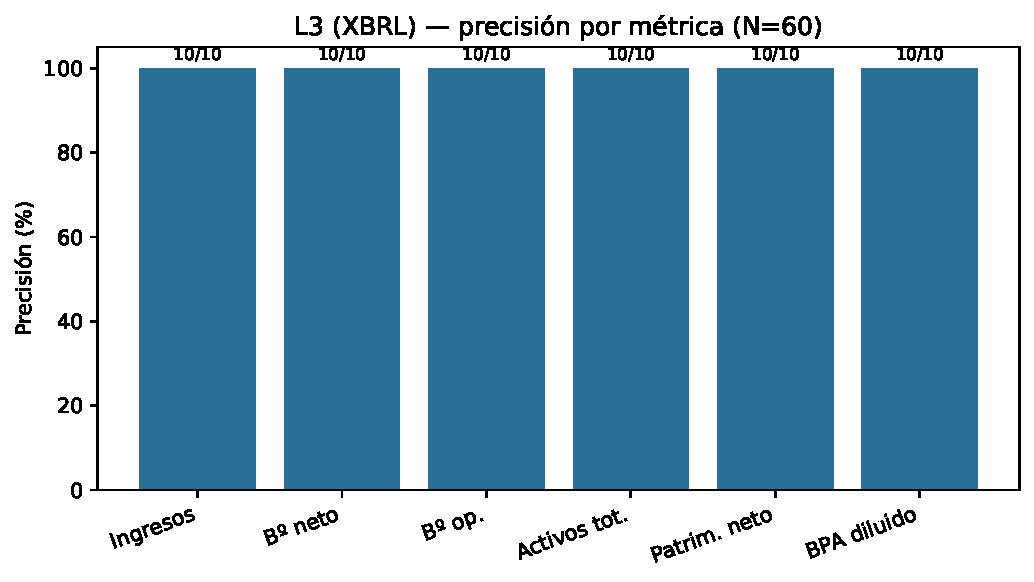
\includegraphics[width=0.95\linewidth]{fig_l3_accuracy_by_metric.pdf}
\caption{Precisión de L3 (extracción estructurada vía XBRL) por métrica
($N=60$). Cada barra anota las coincidencias sobre el total.}
\label{fig:l3acc}
\end{figure}

\begin{figure*}[t]
\centering
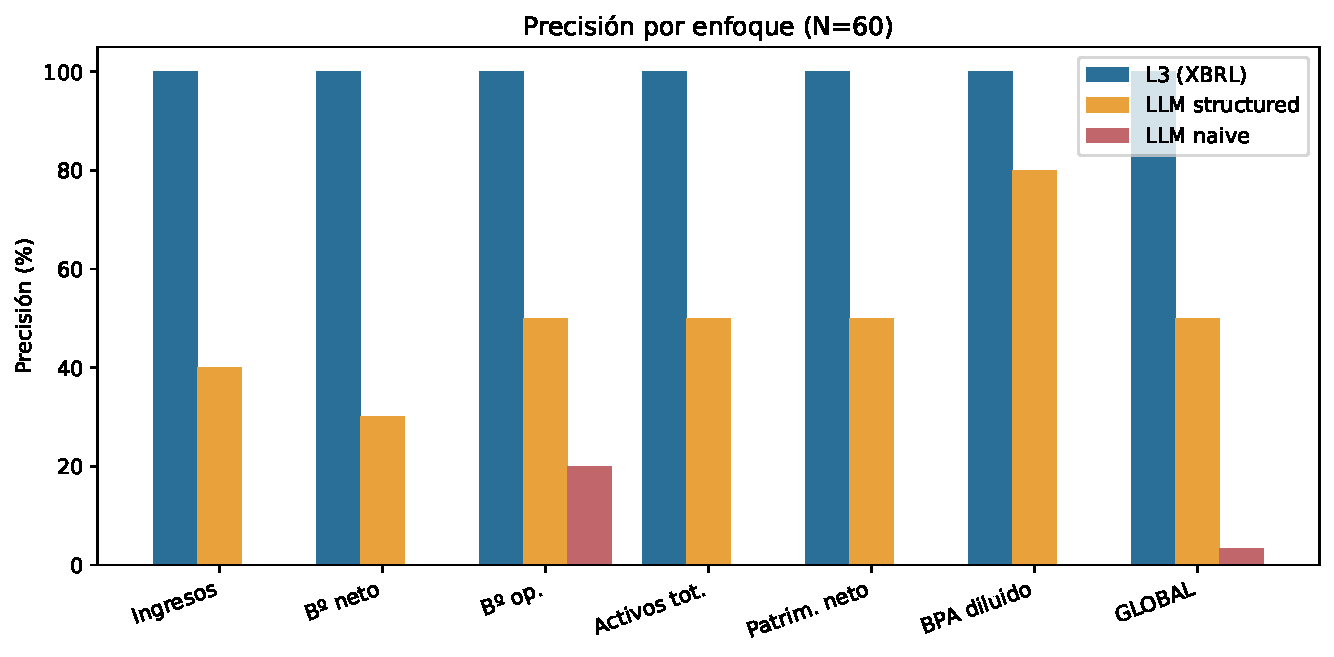
\includegraphics[width=0.92\linewidth]{fig_approach_comparison.pdf}
\caption{Precisión por enfoque: XBRL híbrido (L3) frente a los baselines LLM
\textit{structured} y \textit{naive}, por métrica y en agregado (GLOBAL).}
\label{fig:compare}
\end{figure*}

\subsection{Resultado agregado}
L3 alcanza un \textbf{100\% (60/60)} de precisión, de forma determinista.
El baseline \textit{structured} se sitúa en el \textbf{50.0\%} en la ejecución
reportada (51.7\% en una ejecución previa con el mismo gold), y el baseline
\textit{naive} en un \textbf{3.3\% (2/60)}. La brecha entre L3 y el mejor
baseline es de $\approx$48--50\,pp, y entre L3 y el ingenuo, de
$\approx$96--97\,pp. Esta diferencia es el resultado central del trabajo: las
cifras no deben dejarse en manos de un modelo de 7B.

La precisión de L3 pasó de un 98.3\% en una iteración previa a un 100\% tras
resolver el único fallo pendiente: el beneficio operativo de JNJ, que el emisor no
publica como subtotal. Al anotarlo como nulo y devolver L3 también nulo gracias al
\textit{guard} de recencia, la coincidencia es legítima y no un ajuste
\textit{ad hoc} de los datos. La brecha entre el baseline \textit{structured} y el
\textit{naive} es a su vez de $\approx$47\,pp, lo que sitúa el aporte de
seleccionar tablas financieras (frente a una ventana ciega del texto) en un orden
de magnitud comparable al aporte de XBRL sobre las tablas.

\subsection{Análisis por métrica}
El patrón por métrica es informativo. El baseline \textit{naive} no extrae
\emph{ninguna} cifra correcta de forma genuina: sus dos únicas coincidencias son
casos de beneficio operativo nulo en un banco y un conglomerado
(\textit{null}$=$\textit{null}), por lo que su señal efectiva es $\approx$0\%.
La causa es estructural: con una ventana \textit{head+tail}, el estado de
resultados consolidado, que vive hacia la mitad del documento, queda fuera de
contexto en casi todas las empresas del corpus.

El baseline \textit{structured} se comporta mejor en métricas de presentación
estandarizada. El BPA diluido es la métrica más robusta (80\%): es
invariablemente la última línea del estado de resultados, con formato
\texttt{\$X.XX} y etiqueta ``\textit{Diluted}'', y el modelo la identifica con
fiabilidad. En cambio, ingresos y beneficio neto caen al 30--40\%: el modo de
fallo dominante es la confusión columnar cuando el estado presenta tres
ejercicios en columnas adyacentes sin encabezados claros por columna, y la
ambigüedad entre cifras consolidadas y atribuibles. L3 no sufre ninguno de estos
problemas porque cada \textit{fact} XBRL lleva su periodo, su unidad y su
contexto explícitos.

\subsection{Análisis por empresa y decisiones de anotación}
El comportamiento agregado oculta patrones por empresa que conviene explicitar,
porque informan tanto de la fiabilidad de L3 como de los modos de fallo de los
baselines.

\textbf{Confusión multi-ejercicio en \textit{structured}.} El fallo persistente
del baseline \textit{structured} no se explica por el tamaño bruto del documento:
JPM tiene el HTML más grande del corpus y \textit{structured} acierta 5 de 6
métricas, mientras que KO, con un Item~8 de mayor tamaño, falla 5 de 6. La
dimensión relevante es la \emph{densidad multi-ejercicio} del estado de
resultados: GOOGL, META y AMZN presentan tres ejercicios en columnas adyacentes
sin encabezados claros por columna, y el modelo alinea sistemáticamente los
valores con el año equivocado. Es el mismo mecanismo que produce la ambigüedad
consolidado/atribuible.

\textbf{Verificación de \textit{fiscal year}.} Antes de comparar, verificamos que
el ejercicio anotado coincide con el que descarga L3 en cada par
(\textit{ticker}, métrica). No se detectó desfase temporal: NVDA y WMT se anotan
en FY2026 y el resto en FY2025, en concordancia con los \textit{filings}
cacheados.

\textbf{Decisiones de criterio en el \textit{gold standard}.} Dos casos exigieron
una decisión documentada. En WMT, el beneficio neto se fijó en la cifra
atribuible (no la consolidada con intereses minoritarios) por consistencia con la
convención del BPA, que L3 extrae de \texttt{EarningsPerShareDiluted}. En JNJ y
JPM, el beneficio operativo se anota como nulo porque el emisor no publica ese
subtotal en su estado de resultados; L3 también devuelve nulo gracias al
\textit{guard} de recencia, que descarta un \textit{fact} antiguo de
\texttt{OperatingIncomeLoss}, de modo que la coincidencia
\textit{null}$=$\textit{null} es legítima. Estas decisiones son independientes
del sistema: el \textit{ground truth} se ancla en el documento, no en la salida
de ningún agente.

\section{Discusión}
\label{sec:discussion}
\subsection{Por qué la extracción estructurada gana}
La brecha de $\approx$48--50\,pp confirma que el problema de la extracción
numérica es de \emph{fiabilidad}, no de comprensión. El modelo de 7B
``entiende'' qué es el beneficio neto, pero no lo localiza ni lo copia de forma
consistente en un documento largo y densamente tabular. XBRL resuelve el problema
en el origen: la cifra ya viene etiquetada semánticamente por el emisor. La
arquitectura híbrida pone así cada componente donde es fuerte.

El fracaso casi total del baseline \textit{naive} (3.3\%) tiene una causa
geométrica además de cognitiva. El estado de resultados consolidado de Apple, por
ejemplo, comienza alrededor del carácter 139.000 de un texto plano de unos
220.000; con una ventana \textit{head+tail} de 5.000$+$35.000 caracteres, la zona
central donde viven las cifras del ejercicio más reciente queda sistemáticamente
fuera de contexto. Ampliar la ventana no es una opción en 8\,GB de VRAM. Esto
refuerza el argumento: sin acceso estructurado a los datos, un 7B local no solo
puede equivocarse al leer, sino que con frecuencia ni siquiera \emph{ve} la cifra
correcta.

En el otro extremo, la estabilidad del BPA diluido en el baseline
\textit{structured} (80\%) es instructiva: cuando una magnitud tiene una
presentación fuertemente estandarizada (última línea del estado, formato
\texttt{\$X.XX}, etiqueta ``\textit{Diluted}''), el modelo la identifica de forma
fiable con independencia de cuántos ejercicios aparezcan. La fiabilidad del LLM en
extracción numérica no es uniforme, sino una función de la regularidad de la
presentación; XBRL elimina esa dependencia.

\subsection{Generalización del principio híbrido}
Aunque LUCA se evalúa sobre informes 10-K, el principio que lo vertebra no es
específico de las finanzas: en cualquier dominio donde coexistan datos
estructurados fiables (una base de datos, un formato etiquetado, una API
canónica) y texto no estructurado que requiera interpretación, conviene resolver
lo estructurado con código determinista y reservar el modelo de lenguaje para lo
que solo el lenguaje puede capturar. La aportación metodológica del trabajo no es
un \textit{prompt} ni un modelo concretos, sino la disciplina de trazar y evaluar
esa frontera. El hecho de que la misma arquitectura multiagente provenga de un
sistema de revisión sistemática en otro dominio refuerza esta lectura: lo que
generaliza es la separación de responsabilidades, por encima de los detalles de
implementación.

\subsection{Implicaciones prácticas}
Para un equipo que quiera desplegar análisis financiero asistido por IA sin enviar
datos a terceros ni asumir coste por consulta, los resultados tienen una lectura
directa. Primero, las cifras de un informe deben extraerse del dato estructurado
(XBRL) siempre que exista, no pedírselas al modelo: el ahorro en errores es de
decenas de puntos porcentuales y, además, gratuito y determinista. Segundo, un
modelo de 7B local es suficiente para la capa cualitativa si se le entregan
fragmentos acotados y se acepta una calidad de prosa moderada; no hace falta un
modelo de frontera para producir un borrador útil que un analista revise. Tercero,
la trazabilidad debe construirse en el sistema, no en el modelo: las citas
literales, los identificadores deterministas y los artefactos intermedios
auditables son los que permiten confiar en la salida y revisarla. Estas tres
decisiones, más que cualquier ajuste de \textit{prompt}, son las que determinan si
el sistema es fiable.

\subsection{Techo de calidad del modelo de 7B}
En la capa cualitativa, el mismo modelo de 7B produce un memo legible en español
con cifras exactas (deterministas) y un análisis de riesgos fundamentado en lo
extraído. Su calidad de prosa es limitada y se reporta como una limitación
honesta, no se sustituye por un modelo mayor o externo: la restricción de
hardware de consumo es parte de la tesis del trabajo.

\subsection{La sobre-extracción de riesgos no es uniforme}
\begin{figure*}[t]
\centering
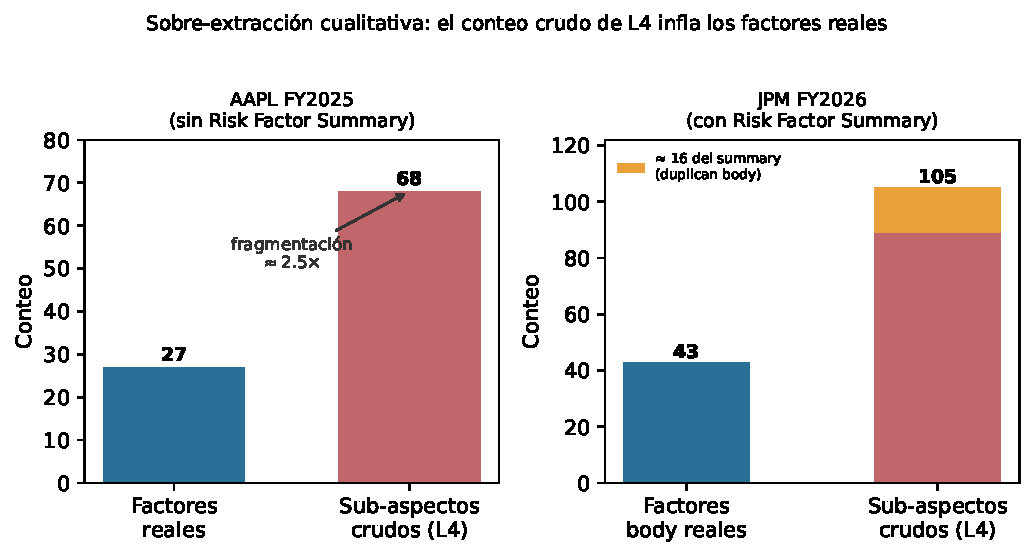
\includegraphics[width=0.82\linewidth]{fig_overextraction.pdf}
\caption{La validación manual de la extracción de riesgos (L4) frente a los
informes muestra que el conteo crudo sobre-estima los factores de riesgo reales,
mediante dos mecanismos distintos según la estructura del documento.}
\label{fig:overext}
\end{figure*}

La validación manual de la salida de L4 contra los informes originales revela
que el conteo crudo de riesgos sobre-estima el número de factores reales, y que
lo hace por dos mecanismos distintos según la estructura del documento
(Fig.~\ref{fig:overext}).

En el 10-K de Apple (FY2025), que \emph{no} incluye un \textit{Risk Factor
Summary}, el inflado es \emph{pura fragmentación del cuerpo}: los 27 factores de
riesgo reales (los 27 encabezados en negrita; las cinco \emph{categorías} quedan
aisladas y no generan riesgos) se descomponen en 68 sub-aspectos extraídos
($\approx$2.5$\times$). El extractor produjo al menos un riesgo para 26 de los 27
factores; el factor de procedimientos legales quedó sin riesgos, lo que es una
limitación del extractor, no una carencia del documento. Por tanto, ``26'' es la
\emph{cobertura} del extractor, no un conteo de factores.

En el 10-K de JPMorgan (FY2026), que \emph{sí} publica un \textit{Risk Factor
Summary}, aparece un segundo mecanismo, la \emph{contaminación
\textit{summary}$\leftrightarrow$\textit{body}}: de los bloques estructurales, 13
pertenecen al resumen y un conteo ingenuo los trataría como factores, y el propio
resumen está además fragmentado (su único \textit{bullet} ``Operational'' generó
seis sub-riesgos). Al excluir los bloques del resumen y un bloque huérfano previo,
quedan 43 factores reales de cuerpo. Alrededor de 16 riesgos derivados del resumen
duplican factores del cuerpo. La Tabla~\ref{tab:overext} resume ambos casos.

\begin{table}[t]
\centering
\caption{Sobre-extracción de riesgos validada manualmente. En AAPL, 27 factores
reales frente a 68 sub-aspectos crudos ($\approx$2.5$\times$); ``26/27'' es la
cobertura del extractor. En JPM, 43 factores de cuerpo frente a 105 crudos, con
$\approx$16 riesgos del \textit{summary} que duplican el cuerpo.}
\label{tab:overext}
\small
\begin{tabular}{@{}lccp{0.34\columnwidth}@{}}
\toprule
Emisor & Factores & Cobertura & Modo de inflado \\
\midrule
AAPL & 27 (de 68) & 26/27 & fragmentación \\
JPM & 43 (de 105) & --- & fragm.\ +\ contam.\ \textit{summary} \\
\bottomrule
\end{tabular}
\end{table}

El valor ``26'' de AAPL es la cobertura del extractor (cuántos de los 27 factores
recibieron al menos un riesgo), no un conteo de factores; lo mantenemos separado
de forma deliberada para no confundir una limitación del extractor con la
estructura del documento.

\subsection{Limitaciones}
La Tabla~\ref{tab:limits} resume las limitaciones del estado actual y su
implicación. Más allá de ellas, conviene subrayar que la evaluación cuantitativa
cubre la capa numérica (L3) y no todavía la calidad de la capa cualitativa, que
se ha validado de forma manual y se documenta como pendiente de evaluación
sistemática.
% TODO(human): frase añadida en T5.2 a partir del corpus (hueco sistemático).
El corpus S\&P~100 revela además un hueco sistemático: el subtotal de beneficio
operativo no se etiqueta en XBRL ni en las financieras (por convención de
presentación) ni en buena parte de farmacéuticas y energéticas, lo que limita la
cobertura de \texttt{operating\_income} en el corpus
(Tabla~\ref{tab:corpus-metric}).

\begin{table}[t]
\centering
\caption{Limitaciones del estado actual e implicación.}
\label{tab:limits}
\begin{tabular}{p{0.30\columnwidth}p{0.58\columnwidth}}
\toprule
Limitación & Implicación \\
\midrule
Sobre-extracción de riesgos & El conteo crudo de L4 infla los factores reales
($\approx$2.5$\times$ en AAPL); requiere una capa de deduplicación. \\
Contaminación de \textit{summary} & En emisores con \textit{Risk Factor Summary}
hay duplicación \textit{summary}$\leftrightarrow$\textit{body}. \\
Calidad de prosa del 7B & Limitada; reportada como restricción de hardware, no
corregida con un modelo mayor. \\
No determinismo del LLM & Los baselines y la capa cualitativa varían entre
ejecuciones; L3 es determinista. \\
Cobertura de categorías & Reputación y conducta no están entre las seis
categorías del config. \\
Solo HTML de EDGAR & No se cubren los PDF no estructurados (p.\,ej. CNMV). \\
\bottomrule
\end{tabular}
\end{table}

\subsection{Amenazas a la validez}
El \textit{gold standard} cubre diez emisores estadounidenses de gran
capitalización; los resultados podrían no generalizar a empresas pequeñas, a
sectores con taxonomías XBRL atípicas o a jurisdicciones distintas. La precisión
de L3 depende además de la completitud y corrección del XBRL que el emisor deposita
en EDGAR; un \textit{filing} con etiquetado deficiente degradaría la extracción sin
que el sistema lo advierta. La evaluación cuantitativa se limita a seis métricas
\textit{core}; \texttt{cash} y \texttt{long\_term\_debt}, ya extraídas por el
código, no se han anotado y quedan fuera del $N=60$. Finalmente, la comparación de
baselines usa un único modelo (Qwen~2.5 7B) y una única GPU; no exploramos otros
modelos de tamaño equivalente, por coherencia con la tesis de hardware de consumo.

\subsection{Reproducibilidad}
L3 es totalmente determinista (XBRL, sin LLM): su 100\% no tiene varianza. Los
baselines LLM y la capa cualitativa no son deterministas por \textit{seed},
porque el cliente de Ollama no propaga la semilla; cabe esperar una variación de
$\pm1$--2 filas entre ejecuciones en los baselines. Por ello reportamos la
brecha como un rango ($\approx$48--50\,pp) y no como un valor exacto. Las cifras
de las tablas y figuras se regeneran desde los CSV de evaluación mediante un
único script, lo que garantiza que el texto y los gráficos no diverjan.

\section{Trabajo futuro}
\label{sec:future}
El análisis de sobre-extracción motiva una \textbf{capa de deduplicación} entre
L4 y L5 con dos responsabilidades, para las cuales la salida actual ya aporta las
señales necesarias: (i)~\emph{mapear los sub-aspectos extraídos a los encabezados
en negrita} (los anclajes del \textit{chunker}), de modo que la fragmentación del
cuerpo colapse a una entrada por factor real; y (ii)~\emph{detectar y descartar el
bloque \textit{Risk Factor Summary}} cuando exista, usando la marca
\texttt{in\_summary} ya disponible, para que los \textit{bullets} del resumen no
se cuenten como factores ni dupliquen el cuerpo. La fragmentación ocurre en todo
emisor, mientras que la contaminación \textit{summary}$\leftrightarrow$\textit{body}
solo aparece en quienes publican un resumen.

Más allá de la deduplicación, la calidad de la capa cualitativa requiere una
\textbf{evaluación sistemática} que en este trabajo solo se ha abordado de forma
manual. Planteamos como línea futura una rúbrica de evaluación del memo (L7) sobre
tres ejes: completitud (cobertura de las secciones esperadas), coherencia interna
y fidelidad al documento fuente, esta última apoyada en las citas literales que
L4 ya conserva. Para la extracción de riesgos (L4) y su clasificación (L5),
proponemos medir precisión y exhaustividad contra un \textit{gold standard}
cualitativo anotado por un humano, análogo al numérico, una vez que la capa de
deduplicación estabilice el conteo de factores. El diagnóstico de los casos sin
clasificar es además accionable: parte de ellos refleja un \emph{gap} de cobertura
del vocabulario (reputación y conducta no están entre las seis categorías), que se
corrige ampliando el conjunto, y parte es inestabilidad de la salida en lote, que
se corrige reduciendo el tamaño de lote.

Quedan también como líneas futuras: la extracción de \textit{forward-looking
statements} y el análisis de tono directivo (fuera del alcance de L4 en esta
iteración); los agentes L6 (comparables) y L8 (\textit{explainability} en Excel);
la anotación y evaluación de las métricas \texttt{cash} y \texttt{long\_term\_debt}
(ya extraídas por L3 a nivel de código, pero no anotadas en el \textit{gold
standard} y, por tanto, fuera del $N=60$); la ampliación del vocabulario de
categorías de riesgo con \textit{reputation} y \textit{conduct}; y el soporte de
PDF no estructurados (p.\,ej. CNMV), que permitiría además estudiar cómo varía la
calidad de extracción entre HTML estructurado y PDF.

\section{Conclusión}
LUCA muestra que una arquitectura híbrida, en la que las cifras provienen de XBRL
y un modelo de 7B local se reserva para lo cualitativo, permite alcanzar una
precisión numérica del 100\% determinista sobre un \textit{gold standard} de 60
puntos de dato, frente al $\approx$50\% del mejor baseline LLM-only y al 3.3\% de
un baseline ingenuo, una brecha de $\approx$48--50\,pp. El sistema completo se
ejecuta en una GPU de consumo de 8\,GB sin recurrir a modelos externos ni APIs de
pago, lo que respalda la viabilidad de la tesis de hardware de consumo. En la capa
cualitativa, el modelo de 7B produce memos utilizables pero con una calidad
limitada y un patrón de sobre-extracción de riesgos que caracterizamos en dos
mecanismos distintos; lo reportamos como límite honesto y como motivación directa
del trabajo futuro, sin sobre-atribuir capacidades al sistema.

La lectura más amplia del trabajo es que, en dominios documentales con datos
estructurados disponibles, la pregunta relevante no es ``¿qué modelo de lenguaje
usar?'' sino ``¿qué parte del problema no debería resolver el modelo de
lenguaje?''. Responderla con una frontera explícita y medible entre lo
determinista y lo generativo es lo que permite que un modelo de 7B en una GPU de
consumo entregue resultados de grado experto en la parte numérica, al tiempo que
se reconocen con honestidad los límites de su parte cualitativa. Esa combinación,
precisión verificable donde el dato lo permite y transparencia sobre las
limitaciones donde no, es un camino practicable para desplegar análisis financiero
asistido por IA sin depender de modelos cerrados de gran escala.

% TODO(human): apéndice de cobertura del corpus (T5.2); tablas
% auto-generadas desde experiments/corpus_manifest.csv por
% experiments/make_corpus_tables.py. Revisar ubicación/estilo.
\appendix
\section{Cobertura del corpus S\&P 100}
\label{sec:appendix-corpus}
Las Tablas~\ref{tab:corpus-metric} y~\ref{tab:corpus-sector} desglosan la
cobertura de campos del corpus (\corpusFilings{} \textit{filings} 10-K,
\corpusCompanies{} empresas, FY2022--FY2024) por métrica \textit{core} y
por sector (división SIC). Cobertura, no accuracy: la accuracy se mide
únicamente contra el gold standard de $N=60$.
% AUTO-GENERATED by experiments/make_corpus_tables.py — do not edit by hand.
% Source: corpus_manifest.csv (288 rows, 96 companies).

\begin{table}[t]
\centering
\caption{Cobertura de campos del corpus S\&P~100 por métrica (288 filings 10-K, 96 empresas, FY2022--FY2024). Cobertura, no accuracy: la accuracy se mide solo contra el gold standard $N=60$.}
\label{tab:corpus-metric}
\begin{tabular}{lrl}
\toprule
Métrica & Cobertura & Motivo dominante de null \\
\midrule
Ingresos & 100.0\% & -- \\
Bº neto & 100.0\% & -- \\
Bº op. & 76.0\% & no aplicable (convención) \\
Activos tot. & 100.0\% & -- \\
Patrim. neto & 100.0\% & -- \\
BPA diluido & 97.9\% & tag ausente \\
\midrule
\textbf{Global} & \textbf{95.7\%} & \\
\bottomrule
\end{tabular}
\end{table}

\begin{table}[t]
\centering
\caption{Cobertura de campos del corpus por sector (división SIC).}
\label{tab:corpus-sector}
\begin{tabular}{lrr}
\toprule
Sector & Filings & Cobertura \\
\midrule
Finanzas, seguros e inmobiliario & 45 & 85.6\% \\
Manufactura & 141 & 96.1\% \\
Comercio minorista & 24 & 100.0\% \\
Servicios & 45 & 98.9\% \\
Transporte, comunicaciones y \textit{utilities} & 33 & 100.0\% \\
\bottomrule
\end{tabular}
\end{table}


\bibliographystyle{IEEEtran}
\bibliography{references}

\end{document}
